%%%::::::::::::::::::::::::::::::scienceThesis V2::::::::::::::::::::::::::::::%%%
%%%::::::::::::::::::::::::::::::scienceThesis V2::::::::::::::::::::::::::::::%%%
%%%:::::::::::::::::::::::::::::::::::::::::::::::::::::::::::::::::::::::::::::::
% Hello!!! Welcome to the \LaTeX{} template for your University of Malta, Faculty 
% of Science thesis. This template was created (hacked!) by 
% William Hicklin B.Sc (Hons) Chem & Phy and Eric Pace B.Sc (Hons) Phy & AI (2012)
%%%:::::::::::::::::::::::::::::::::::::::::::::::::::::::::::::::::::::::::::::::
% This is the preamble code required for part of the thesis type-setting. This
% code must be included before the \begin{document} in the scienceThesis.tex file.
% To do this use the command %%%::::::::::::::::::::::::::::::scienceThesis V2::::::::::::::::::::::::::::::%%%
%%%:::::::::::::::::::::::::::::::::::::::::::::::::::::::::::::::::::::::::::::::
% Hello!!! Welcome to the \LaTeX{} template for your University of Malta, Faculty 
% of Science thesis. This template was created (hacked!) by 
% William Hicklin B.Sc (Hons) Chem & Phy and Eric Pace B.Sc (Hons) Phy & AI (2012)
%%%:::::::::::::::::::::::::::::::::::::::::::::::::::::::::::::::::::::::::::::::
% This is the preamble code required for part of the thesis type-setting. This
% code must be included before the \begin{document} in the scienceThesis.tex file.
% To do this use the command %%%::::::::::::::::::::::::::::::scienceThesis V2::::::::::::::::::::::::::::::%%%
%%%:::::::::::::::::::::::::::::::::::::::::::::::::::::::::::::::::::::::::::::::
% Hello!!! Welcome to the \LaTeX{} template for your University of Malta, Faculty 
% of Science thesis. This template was created (hacked!) by 
% William Hicklin B.Sc (Hons) Chem & Phy and Eric Pace B.Sc (Hons) Phy & AI (2012)
%%%:::::::::::::::::::::::::::::::::::::::::::::::::::::::::::::::::::::::::::::::
% This is the preamble code required for part of the thesis type-setting. This
% code must be included before the \begin{document} in the scienceThesis.tex file.
% To do this use the command \input{Preamble.tex}.
%%%:::::::::::::::::::::::::::::::::::::::::::::::::::::::::::::::::::::::::::::::
\documentclass[12pt,a4paper]{report}

\usepackage{packages/scienceThesis}% Needed for further type-settings and commands
\usepackage{verbatim}% needed for the ``code" and other environments
\usepackage{amsfonts}
\usepackage{amsmath}
\usepackage{amssymb}
\usepackage{amsthm}
\usepackage{bibunits}% needed for the bibliography section
\usepackage{lipsum}% needed for the generating text in the example
\usepackage[acronym,toc,nonumberlist]{glossaries}% This package is required for adding acronyms.


%%%:::::::::::::::::::::::::::::::::::::::::::::::::::::::::::::::::::::::::::::::
% The following environments are useful to present proofs in your thesis. These
% packages are not really necessary, if you don't need the code and proofs
% environments, so if you like you can delete from here till ``the next comment".
% Note that there are some examples below which obviously won't work once you
% remove this part
%%%:::::::::::::::::::::::::::::::::::::::::::::::::::::::::::::::::::::::::::::::
\theoremstyle{definition}
\newtheorem{definition}{Definition}[section]
\theoremstyle{definition}%plain}
\newtheorem{example}{Example}[section]
\theoremstyle{definition}%remark}
\newtheorem{proposition}{Proposition}[section]
\theoremstyle{definition}%remark}
\newtheorem{lemma}{Lemma}[section]
\theoremstyle{definition}%remark}
\newtheorem{corollary}{Corollary}[section]
\theoremstyle{definition}%remark}
\newtheorem{theorem}{Theorem}[section]
%%%:::::::::::::::::::::::::::::::::::::::::::::::::::::::::::::::::::::::::::::::
% The next comment!
%%%:::::::::::::::::::::::::::::::::::::::::::::::::::::::::::::::::::::::::::::::

%%%:::::::::::::::::::::::::::::::::::::::::::::::::::::::::::::::::::::::::::::::
% This section customises the headers of chapters, headers and footers.
%%%:::::::::::::::::::::::::::::::::::::::::::::::::::::::::::::::::::::::::::::::
% Customising headers and footers.
%:::::::::::::::::::::::::::::::::::::::::::::::::::::::::::::::::::::::::::::::::
\usepackage{fancyhdr}
\pagestyle{fancy}
\rhead{}
\lhead{\nouppercase{\textsc{\leftmark}}}
\renewcommand{\headrulewidth}{1pt}
\makeatletter
\renewcommand{\chaptermark}[1]{\markboth{\small\textsc{\@chapapp}\ \thechapter:\ \sc{#1}}{}}
\makeatother
%:::::::::::::::::::::::::::::::::::::::::::::::::::::::::::::::::::::::::::::::::
% Customising chapter headings.
%:::::::::::::::::::::::::::::::::::::::::::::::::::::::::::::::::::::::::::::::::
\usepackage{sectsty}
\chapterfont{\large\sc\centering}
\chaptertitlefont{\sc\centering}
\subsubsectionfont{\centering}
%%%:::::::::::::::::::::::::::::::::::::::::::::::::::::::::::::::::::::::::::::::


%%%:::::::::::::::::::::::::::::::::::::::::::::::::::::::::::::::::::::::::::::::
% PDF hyper-linking (set colours to black for printing)
%%%:::::::::::::::::::::::::::::::::::::::::::::::::::::::::::::::::::::::::::::::
\usepackage[colorlinks]{hyperref}
%\usepackage[figure,table]{hypcap}
\hypersetup{
	bookmarksnumbered,
	pdfstartview={FitH},
	citecolor={black},
	linkcolor={black},
	urlcolor={black},
	pdfpagemode={UseOutlines}
}
%%%:::::::::::::::::::::::::::::::::::::::::::::::::::::::::::::::::::::::::::::::
\setlength{\headheight}{15pt}


%%%:::::::::::::::::::::::::::::::::::::::::::::::::::::::::::::::::::::::::::::::
% Sets the document to be line separated paragraphs not indentation separated
% paragraphs. To change to an indentation with no line skip simply change
% \parindent 0cm --> \parindent 1.3cm & \parskip 2ex --> \parskip 0ex
%%%:::::::::::::::::::::::::::::::::::::::::::::::::::::::::::::::::::::::::::::::
\parindent 0cm
\parskip 2ex

\makeglossaries

%%%:::::::::::::::::::::::::::::::::::::::::::::::::::::::::::::::::::::::::::::::
% End of preamble
%%%:::::::::::::::::::::::::::::::::::::::::::::::::::::::::::::::::::::::::::::::.
%%%:::::::::::::::::::::::::::::::::::::::::::::::::::::::::::::::::::::::::::::::
\documentclass[12pt,a4paper]{report}

\usepackage{packages/scienceThesis}% Needed for further type-settings and commands
\usepackage{verbatim}% needed for the ``code" and other environments
\usepackage{amsfonts}
\usepackage{amsmath}
\usepackage{amssymb}
\usepackage{amsthm}
\usepackage{bibunits}% needed for the bibliography section
\usepackage{lipsum}% needed for the generating text in the example
\usepackage[acronym,toc,nonumberlist]{glossaries}% This package is required for adding acronyms.


%%%:::::::::::::::::::::::::::::::::::::::::::::::::::::::::::::::::::::::::::::::
% The following environments are useful to present proofs in your thesis. These
% packages are not really necessary, if you don't need the code and proofs
% environments, so if you like you can delete from here till ``the next comment".
% Note that there are some examples below which obviously won't work once you
% remove this part
%%%:::::::::::::::::::::::::::::::::::::::::::::::::::::::::::::::::::::::::::::::
\theoremstyle{definition}
\newtheorem{definition}{Definition}[section]
\theoremstyle{definition}%plain}
\newtheorem{example}{Example}[section]
\theoremstyle{definition}%remark}
\newtheorem{proposition}{Proposition}[section]
\theoremstyle{definition}%remark}
\newtheorem{lemma}{Lemma}[section]
\theoremstyle{definition}%remark}
\newtheorem{corollary}{Corollary}[section]
\theoremstyle{definition}%remark}
\newtheorem{theorem}{Theorem}[section]
%%%:::::::::::::::::::::::::::::::::::::::::::::::::::::::::::::::::::::::::::::::
% The next comment!
%%%:::::::::::::::::::::::::::::::::::::::::::::::::::::::::::::::::::::::::::::::

%%%:::::::::::::::::::::::::::::::::::::::::::::::::::::::::::::::::::::::::::::::
% This section customises the headers of chapters, headers and footers.
%%%:::::::::::::::::::::::::::::::::::::::::::::::::::::::::::::::::::::::::::::::
% Customising headers and footers.
%:::::::::::::::::::::::::::::::::::::::::::::::::::::::::::::::::::::::::::::::::
\usepackage{fancyhdr}
\pagestyle{fancy}
\rhead{}
\lhead{\nouppercase{\textsc{\leftmark}}}
\renewcommand{\headrulewidth}{1pt}
\makeatletter
\renewcommand{\chaptermark}[1]{\markboth{\small\textsc{\@chapapp}\ \thechapter:\ \sc{#1}}{}}
\makeatother
%:::::::::::::::::::::::::::::::::::::::::::::::::::::::::::::::::::::::::::::::::
% Customising chapter headings.
%:::::::::::::::::::::::::::::::::::::::::::::::::::::::::::::::::::::::::::::::::
\usepackage{sectsty}
\chapterfont{\large\sc\centering}
\chaptertitlefont{\sc\centering}
\subsubsectionfont{\centering}
%%%:::::::::::::::::::::::::::::::::::::::::::::::::::::::::::::::::::::::::::::::


%%%:::::::::::::::::::::::::::::::::::::::::::::::::::::::::::::::::::::::::::::::
% PDF hyper-linking (set colours to black for printing)
%%%:::::::::::::::::::::::::::::::::::::::::::::::::::::::::::::::::::::::::::::::
\usepackage[colorlinks]{hyperref}
%\usepackage[figure,table]{hypcap}
\hypersetup{
	bookmarksnumbered,
	pdfstartview={FitH},
	citecolor={black},
	linkcolor={black},
	urlcolor={black},
	pdfpagemode={UseOutlines}
}
%%%:::::::::::::::::::::::::::::::::::::::::::::::::::::::::::::::::::::::::::::::
\setlength{\headheight}{15pt}


%%%:::::::::::::::::::::::::::::::::::::::::::::::::::::::::::::::::::::::::::::::
% Sets the document to be line separated paragraphs not indentation separated
% paragraphs. To change to an indentation with no line skip simply change
% \parindent 0cm --> \parindent 1.3cm & \parskip 2ex --> \parskip 0ex
%%%:::::::::::::::::::::::::::::::::::::::::::::::::::::::::::::::::::::::::::::::
\parindent 0cm
\parskip 2ex

\makeglossaries

%%%:::::::::::::::::::::::::::::::::::::::::::::::::::::::::::::::::::::::::::::::
% End of preamble
%%%:::::::::::::::::::::::::::::::::::::::::::::::::::::::::::::::::::::::::::::::.
%%%:::::::::::::::::::::::::::::::::::::::::::::::::::::::::::::::::::::::::::::::
\documentclass[12pt,a4paper]{report}

\usepackage{packages/scienceThesis}% Needed for further type-settings and commands
\usepackage{verbatim}% needed for the ``code" and other environments
\usepackage{amsfonts}
\usepackage{amsmath}
\usepackage{amssymb}
\usepackage{amsthm}
\usepackage{bibunits}% needed for the bibliography section
\usepackage{lipsum}% needed for the generating text in the example
\usepackage[acronym,toc,nonumberlist]{glossaries}% This package is required for adding acronyms.


%%%:::::::::::::::::::::::::::::::::::::::::::::::::::::::::::::::::::::::::::::::
% The following environments are useful to present proofs in your thesis. These
% packages are not really necessary, if you don't need the code and proofs
% environments, so if you like you can delete from here till ``the next comment".
% Note that there are some examples below which obviously won't work once you
% remove this part
%%%:::::::::::::::::::::::::::::::::::::::::::::::::::::::::::::::::::::::::::::::
\theoremstyle{definition}
\newtheorem{definition}{Definition}[section]
\theoremstyle{definition}%plain}
\newtheorem{example}{Example}[section]
\theoremstyle{definition}%remark}
\newtheorem{proposition}{Proposition}[section]
\theoremstyle{definition}%remark}
\newtheorem{lemma}{Lemma}[section]
\theoremstyle{definition}%remark}
\newtheorem{corollary}{Corollary}[section]
\theoremstyle{definition}%remark}
\newtheorem{theorem}{Theorem}[section]
%%%:::::::::::::::::::::::::::::::::::::::::::::::::::::::::::::::::::::::::::::::
% The next comment!
%%%:::::::::::::::::::::::::::::::::::::::::::::::::::::::::::::::::::::::::::::::

%%%:::::::::::::::::::::::::::::::::::::::::::::::::::::::::::::::::::::::::::::::
% This section customises the headers of chapters, headers and footers.
%%%:::::::::::::::::::::::::::::::::::::::::::::::::::::::::::::::::::::::::::::::
% Customising headers and footers.
%:::::::::::::::::::::::::::::::::::::::::::::::::::::::::::::::::::::::::::::::::
\usepackage{fancyhdr}
\pagestyle{fancy}
\rhead{}
\lhead{\nouppercase{\textsc{\leftmark}}}
\renewcommand{\headrulewidth}{1pt}
\makeatletter
\renewcommand{\chaptermark}[1]{\markboth{\small\textsc{\@chapapp}\ \thechapter:\ \sc{#1}}{}}
\makeatother
%:::::::::::::::::::::::::::::::::::::::::::::::::::::::::::::::::::::::::::::::::
% Customising chapter headings.
%:::::::::::::::::::::::::::::::::::::::::::::::::::::::::::::::::::::::::::::::::
\usepackage{sectsty}
\chapterfont{\large\sc\centering}
\chaptertitlefont{\sc\centering}
\subsubsectionfont{\centering}
%%%:::::::::::::::::::::::::::::::::::::::::::::::::::::::::::::::::::::::::::::::


%%%:::::::::::::::::::::::::::::::::::::::::::::::::::::::::::::::::::::::::::::::
% PDF hyper-linking (set colours to black for printing)
%%%:::::::::::::::::::::::::::::::::::::::::::::::::::::::::::::::::::::::::::::::
\usepackage[colorlinks]{hyperref}
%\usepackage[figure,table]{hypcap}
\hypersetup{
	bookmarksnumbered,
	pdfstartview={FitH},
	citecolor={black},
	linkcolor={black},
	urlcolor={black},
	pdfpagemode={UseOutlines}
}
%%%:::::::::::::::::::::::::::::::::::::::::::::::::::::::::::::::::::::::::::::::
\setlength{\headheight}{15pt}


%%%:::::::::::::::::::::::::::::::::::::::::::::::::::::::::::::::::::::::::::::::
% Sets the document to be line separated paragraphs not indentation separated
% paragraphs. To change to an indentation with no line skip simply change
% \parindent 0cm --> \parindent 1.3cm & \parskip 2ex --> \parskip 0ex
%%%:::::::::::::::::::::::::::::::::::::::::::::::::::::::::::::::::::::::::::::::
\parindent 0cm
\parskip 2ex

\makeglossaries

%%%:::::::::::::::::::::::::::::::::::::::::::::::::::::::::::::::::::::::::::::::
% End of preamble
%%%:::::::::::::::::::::::::::::::::::::::::::::::::::::::::::::::::::::::::::::::

\usepackage[version=3]{mhchem}% usage \ce{CO2}, \ce{2H2 + O2 -> 2H2O} etc.
\usepackage{siunitx}% usage \SI{number}{units} or \si{units}. Separate different SI units by . e.x. m.s^-1
\usepackage{url}% usage \url{write your url as is}

\begin{document}

%%%:::::::::::::::::::::::::::::::::::::::::::::::::::::::::::::::::::::::::::::::
% The following fields are required information to be filled for the thesis.
%%%:::::::::::::::::::::::::::::::::::::::::::::::::::::::::::::::::::::::::::::::
\title{Dissertation Title}
\author{name surname}
\date{Publication date}
\supervisor{supervisor}
\department{Physics}% Physics, Chemistry or Biology
\degree{M.Sc}% B.Sc (Hons), M.Sc, Ph.D


%%%:::::::::::::::::::::::::::::::::::::::::::::::::::::::::::::::::::::::::::::::
% The following fields are optional although certain fields, e.x. abstract,
% acknowledgements, are must to be filled for the final dissertation.
%%%:::::::::::::::::::::::::::::::::::::::::::::::::::::::::::::::::::::::::::::::
\cosupervisor{cosupervisor}
\acronyms{acronyms}% Enter the tex file containing the acronym information.
\dedication{\textbf{To Eiichiro Oda}\\For fuelling my motivation through epic tales}
\acknowledgements{
Write your acknowledgements within these curly brackets. To clear and skip lines you will have the use the double backslash command.\\
\\
If you take a look at science in its everyday function, of course you find that scientists run the gamut of human emotions and personalities and character and so on. But there's one thing that is really striking to the outsider, and that is the gauntlet of criticism that is considered acceptable or even desirable. The poor graduate student at his or her Ph.D. oral exam is subjected to a withering crossfire of questions that sometimes seem hostile or contemptuous; this from the professors who have the candidate's future in their grasp. The students naturally are nervous; who wouldn't be? True, they've prepared for it for years. But they understand that at that critical moment they really have to be able to answer questions. So in preparing to defend their theses, they must anticipate questions; they have to think,``Where in my thesis is there a weakness that someone else might find because I sure better find it before they do, because if they find it and I'm not prepared, I'm in deep trouble."\\
\\
Carl Sagan}
\abstract{
Write your abstract within these curly brackets. To clear and skip lines you will have the use the double backslash command.\\
\\
After your first job, is anyone asking you what your GPA was? No, they don't care. They ask you: Are you a good leader? Do people follow you? Do you have integrity? Are you innovative? Do you solve problems? Somebody's got to do that homework and redesign the educational system so that it can actually train people to be successful in life.\\
\\
I think the greatest teachers are not the ones that are best trained at educational tactics. I don't know a person who's ever said,``Boy, that teacher is so good! The teacher gives such good exams. That teacher gives such good homework sets!" No one has said that about a great teacher. That's not what people remember about the great teachers they've had.\\
\\
The best educators are the ones that inspire their students. That inspiration comes from a passion that teachers have for the subject they're teaching. Most commonly, that person spent their lives studying that subject, and they bring an infectious enthusiasm to the audience.\\
\\
I think many people have that enthusiasm, but they are prevented from being teachers because they didn't go through the teacher mill. Now you have teachers who have been through the teacher mill, yet they have no capacity to inspire anyone at all. It's the inspired student that continues to learn on their own. That's what separates the real achievers in the world from those who pedal along, finishing assignments.\\
\\
Neil deGrasse Tyson}
\publications{
If you have published and papers during your thesis include them here. BTW... well done!
}
%%%:::::::::::::::::::::::::::::::::::::::::::::::::::::::::::::::::::::::::::::::

\frontmatter% this command will generate all the front pages according to the information entered in the section above. 

\chapter{Introduction}

This template was generated according to the University of Malta, Department of Physics guidelines \cite{guidelines}. In the following chapters some examples regarding the use of this template and other common commands are illustrated. Most of this and other information can be acquired for the \LaTeX{} wiki books\footnote{\url{http://en.wikibooks.org/wiki/LaTeX/}}.

To use abbreviations add the acronyms command with the \textit{acronyms.tex} file between the curly brackets. Add your abbreviations to the \textit{acronyms.tex} file using the command
\begin{code}
\newacronym{label}{abbreviation}{full_name}
e.x
\newacronym{pv}{PV}{Photovoltaic}
\end{code}
When you want to use the abbreviation use the commands

\begin{table}[h!]
\center
\begin{tabular}{l p{11cm}}
\verb|\gls{label}| & This command prints the term associated with $<$label$>$ passed as its argument.\\
\verb|\glspl{<label>}| & This command prints the plural of the defined therm, other than that it behaves in the same way as gls.\\
\verb|\Gls{<label>}| & This command prints the singular form of the term with the first character converted to upper case.\\
\verb|\Glspl{<label>}| & This command prints the plural form with first letter of the term converted to upper case.\\
\end{tabular}
\end{table}

The first time a the acronym is used it is axiomatically written as the full name with the abbreviation in parentheses. The rest of the time it is written as the abbreviation. To generate the acronym page, or refresh it, one has to execute the command

\begin{code}
makeglossaries <fileName>
\end{code}

from the terminal (unix) or cmd (windows). The following paragraph shows an example of how to use acronyms and how they are displayed.

\Glspl{dssc} are \gls{pv} cells using organic materials instead of \glspl{sc}. They usually use nano-particles of \gls{tio2} as a \gls{sc} to transfer electrons \cite{Gra91}.

The rest of the text is lorem ipsum, just to show the type-setting, with the exception of a few example showing you how to use various environments and commands.


\chapter{Lorem Ipsum}

\lipsum[2]

\section{Section}

\lipsum[1-4]

\subsection{Subsection}

\lipsum[1]

\subsubsection{Subsubsection}

\lipsum[1-3]

\section{Section}

\lipsum[1-2]

\chapter{Environments examples}

\section{scienceThesis.sty environments}

\begin{definition}
This is an example of a definition
\end{definition}

\begin{example}
This is an example of an example :)
\end{example}

\begin{proposition}
This is an example of a proposition.
\end{proposition}

\begin{lemma}
This is an example of a lemma.
\end{lemma}

\begin{corollary}
This is an example of a corollary
\end{corollary}

\begin{theorem}
This is an example of a theorem.
\end{theorem}

\begin{proof}
This is an example of a proof.
\end{proof}

\section{\LaTeX{} environments}

Table \ref{tab:ResitanceTable} is an example of both, how to create tables in \LaTeX{} and how to use cross-referencing. Equation \ref{eq:Schr} show the Schr\"{o}dinger equation, an example of how to write equations, and how to cross-reference equations \cite{Quantum}.

\begin{table}[h!]
	\centering
	\begin{tabular}{c | c}
		I & $\Omega$ \\ \hline
		12 & 4 \\
		10 & 6 \\
		8 & 8 \\
		6 & 10 \\
	\end{tabular}
	\caption[short caption]{long caption}% short caption is optional and if filled is used in the table of contents.
	\label{tab:ResitanceTable}
\end{table}

\begin{equation}
i\hbar \frac{\partial \psi}{\partial t} = -\frac{\hbar^2}{2m}\nabla^2 \psi + V(\mathbf{r})
\label{eq:Schr}
\end{equation}

Figure \ref{fig:WordVsLatex} show how to insert graphics in a \LaTeX{} documents and also how to cross-reference it.

\begin{figure}[h!]
\centering
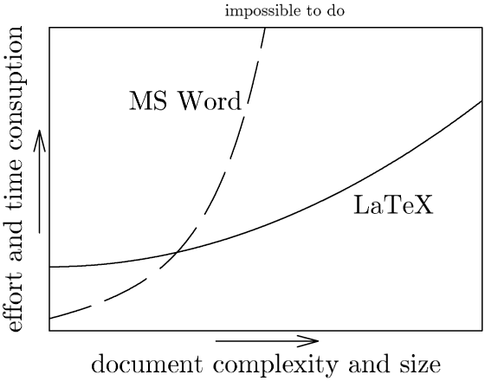
\includegraphics[width=0.6 \textwidth]{pics/WordVsLatex.png}
\caption{A plot show how much easier it is to write documents with \LaTeX{}} \label{fig:WordVsLatex}
\end{figure}

\chapter{Chemistry examples}

The following are examples of how to use the \textit{mhchem} package.

\ce{^{227}_{90}Th+}, \ce{Ce^{IV}}, \ce{KCr(SO4)2.12H2O}, \ce{RNO2^{-.}}

\ce{H2 + 1/2O2 = H2O}

\ce{K3[Fe(CN)6] <=> 3K+ + [Fe(CN)6]-}

\ce{H+ + OH- <=>> H2O}

\ce{NH4NO3 + H2O ->[\Delta] NH4+_{(aq)} + NO3-_{(aq)}}

\ce{X=Y#Z}, \ce{CH3\sbond C\tbond C\dbond CH2}, \ce{A\bond{...}B}

\begin{equation}
\ce{AgCl <=> Ag+ + Cl-}
\end{equation}

\begin{equation}
\ce{CO2 + 6H2O ->[\textcolor{blue}{Light Energy}][\textcolor{red}{Endothermic}] C6H12O6 + CO2 \quad \Delta G^{\circ}} = \SI{+2870}{kJ.mol^{-1}}
\end{equation}

For more information on how to use this package, download ``The mhchem Bundle" pdf. \cite{*}


%%%:::::::::::::::::::::::::::::::::::::::::::::::::::::::::::::::::::::::::::::::
% The following commands are required for generating the references section.
% \bibliographystyle{} command sets the citation style and \bibliography{} gives
% the files in which the bibliography code is place. If the code is contained in
% multiple files, separate them by a comma and NO space e.x. {ref1.bib,ref2.bib}
%
% References and Bibliography should be placed before the Appendix.
%%%:::::::::::::::::::::::::::::::::::::::::::::::::::::::::::::::::::::::::::::::
\bibliomatter
\bibliographystyle{packages/aip}
\bibliography{ref}

%%%:::::::::::::::::::::::::::::::::::::::::::::::::::::::::::::::::::::::::::::::
% The following command will add the bibliography section including all the
% materials who's citation code is written in bib.bib, or the files written
% between the {}.
%%%:::::::::::::::::::::::::::::::::::::::::::::::::::::::::::::::::::::::::::::::
\bibliografia{packages/vancouver}{bib}

\appendix

\chapter{Examples of code environments}

\section{The code environment}

\begin{code}
this is some code;
I hope you found this template useful.
\end{code}

\section{The listings environment}

\begin{minipage}{\textwidth}
\begin{lstlisting}[numbers=left]
BEFOREHAND: close door, each window & exit; wait until time.
    open spellbook, study, read (scan, select, tell us);
write it, print the hex while each watches,
    reverse its length, write again;
    kill spiders, pop them, chop, split, kill them.
        unlink arms, shift, wait & listen (listening, wait),
sort the flock (then, warn the "goats" & kill the "sheep");
    kill them, dump qualms, shift moralities,
    values aside, each one;
        die sheep! die to reverse the system
        you accept (reject, respect);
next step,
    kill the next sacrifice, each sacrifice,
    wait, redo ritual until "all the spirits are pleased";
    do it ("as they say").
do it(*everyone***must***participate***in***forbidden**s*e*x*).
return last victim; package body;
    exit crypt (time, times & "half a time") & close it,
    select (quickly) & warn your next victim;
AFTERWORDS: tell nobody.
    wait, wait until time;
    wait until next year, next decade;
        sleep, sleep, die yourself,
        die at last
# Larry Wall
\end{lstlisting}
\end{minipage}

The above poem/script was written in perl 3 by Larry Wall and is called \textit{black perl} \cite{blackPerl}.

\end{document}